Drift detection of corrupted samples for the problem of the thesis has been performed using \textit{alibi-detect} open source python library, that focuses specifically on outlier, adversarial and drift detection algorithms (\cite{alibi-detect}). This library implements statistical hypothesis testing algorithms for detecting drifts in data. 

It works the following way, before observing some data, one can specify null-hypothesis $H_0$ and alternative hypothesis $H_1$ about generating process behind the data (its distribution for example) and also specify the test statistics $S(X)$ that are expected to be small under hypothesis $H_0$ and large under hypothesis $H_1$. Then during the observation of the new data test statistic value $S(X)$ is computed along with a probability $p = P(S(X)|H_0)$ which is called p-value. P-value is a probability that such an extreme value of test statistic could have been observed under the null-hypothesis. If this probability is below the established threshold $t$, then one can assume that data is drifted. If p-value is low, null-hypothesis will be refused. 

A drift detection algorithm was trained on UNet embeddings of not corrupted train data. For this experiment $10,000$ embeddings were used of CHZN and PHX phenotypes from the nucleus dataset. It is important that the crops were chosen in such a way that at least several cells present are present there. After splitting images into the crops many of them contain a primarily background with few cells present. By filtering out these crops one can make sure that drift detection model actually learns on the important foreground signal from the cells rather than on the predictions of the background. After the drift detection algorithm was trained, it was tested on the dataset, that was not seen by a model beforehand (test dataset). Test dataset consists of $119$ images, where from each image $5$ random crops were chosen. The crops for each image were chosen again in the same way as fro training by only choosing the ones that have enough cells present in them. Since images have a high resolution, one can assume that one image itself represents a new input distribution, where crops taken from this image are its samples. Therefore we can detect whether one specific image has drifted or not feeding the crops from it into a drift detection algorithm. First, the algorithm was tested on not drifted data by using a test set of nucleus dataset. Out of $119$ images $8$ were recognized as drifted ones. This means that the algorithm's false positive is approximately $\frac{8}{119} \approx 0.063$.

Below the results of the trained drift detector for two datasets are presented: same test data with artificial corruptions applied to it and on data with real microscopy corruptions. 

\textbf{Artificial corruptions}

Figure \ref{fig:fn-rate} presents the results of drift detection for all artificial corruptions, more specifically the algorithm's false negative rate.
\begin{figure}[H]
	\begin{center}
		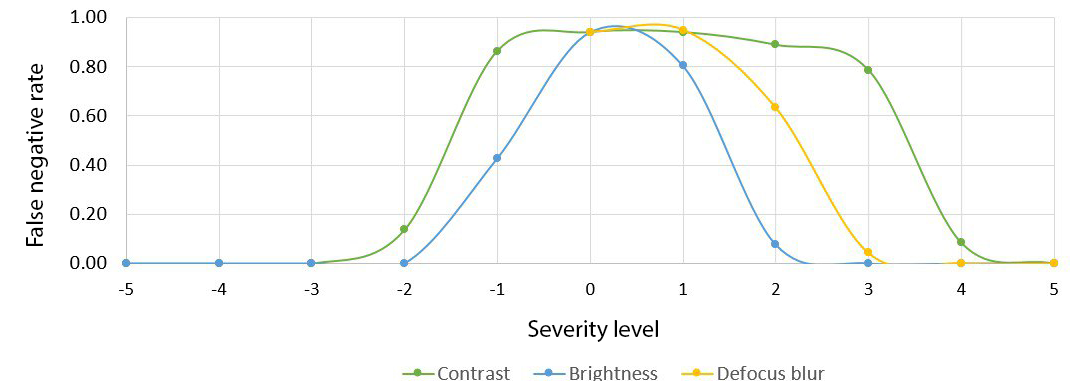
\includegraphics[width=\linewidth]{bilder/drift-detection/fn-rate.png}
		\caption[False negatives rate for drift detection on artificial corruptions]%
		{False negatives rate for drift detection on artificial corruptions- Long Description}{}\label{fig:fn-rate}
	\end{center}
\end{figure}
One can see that the lower the severity of a corruption is, the higher the false negative rate becomes. When the corruption severity level is low the predictions remain to have a high quality (see Figure \ref{fig:artificial-corruptions}), therefore an end user can still rely on the UNet. However, the stronger the corruption is, the stronger fluorescence prediction degenerates and as a result a drift detector alerts a user to the presence of drift. Drift detector is more sensitive towards contrast changes rather then towards defocus blur changes. It is the most sensitive towards brightness corruption.

\textbf{Real corruptions}

Types of real corruptions tested here are described in more details in Section \ref{section:real-corruptions}. Two phenotypes are present there: PHX (was also present in the training dataset) and 2e3 (was not present in any of the datasets before). Since these two subsets of data look very much alike drift detection results on both of them will be combined. In Table \ref{table:real-corruptions-dd} the results of the drift detection algorithm are presented. Additionally, for few samples of not drifted data that were also included in this dataset, namely 2 images of the correct focus distance Z and 4 images of the correct exposure time (30ms), the detector falsely alerted $0$ and $1$ samples correspondingly. The results confirm that the detector is trained well enough to be able to detect drift to some extent, however not all drifted images will be noticed by it. In order to state how exactly accurate it for real corruptions is much more data would be needed. Assuming that uncorrupted test dataset is representative enough, the low false positive rate is expected (around $0.063$). That is why one can presumably rely on the detector to alert the user about wrong exposures or focus corruptions. Regarding wrong fixation time of the cells, on the one hand it seems that this corruption has somewhat low detection rate, on the other one model's predictions are actually of quite a good quality. Therefore it might be the model is generally quite stable towards the prolonged fixation time.

\begin{table}[htb]
    \centering
    \caption{Drift detection for real microscopy corruptions}
        \begin{adjustbox}{width=\textwidth}
            \begin{tabular}{|c||c|c|c|c|c|}\hline
				
                &15 minute fixation
                &-5 Z
                &+5 Z
                &20 ms exposure
                &40 ms exposure
                \\\hline\hline
            	Detections & 3 & 2 & 3 & 2 & 2\\\hline
                Total images & 8 & 4 & 4 & 4 & 4\\\hline
            \end{tabular}
        \end{adjustbox}
    \label{table:real-corruptions-dd}
\end{table}